\documentclass[letterpaper,11pt,oneside,reqno]{article}

%%%%%%%%%%%%%%%%%%%%%%%%%%%%%%%%%%%%%%%%%%%%%%%%%%%%%%%%%%%%

\usepackage[pdftex,backref=page,colorlinks=true,linkcolor=blue,citecolor=red]{hyperref}
\usepackage[alphabetic,nobysame]{amsrefs}

%%%%%%%%%%%%%%%%%%%%%%%%%%%%%%%%%%%%%%%%%%%%%%%%%%%%%%%%%%%%
%main packages
\usepackage{amsmath,amssymb,amsthm,amsfonts,mathtools}
\usepackage{graphicx,color}
\usepackage{upgreek}
\usepackage[mathscr]{euscript}

%equations
\allowdisplaybreaks
\numberwithin{equation}{section}

%tikz
\usepackage{tikz}
\usetikzlibrary{shapes,arrows,positioning,decorations.markings}

%conveniences
\usepackage{array}
\usepackage{adjustbox}
\usepackage{cleveref}
\usepackage{enumerate}
\usepackage{datetime}

%paper geometry
\usepackage[DIV=12]{typearea}

%%%%%%%%%%%%%%%%%%%%%%%%%%%%%%%%%%%%%%%%%%%%%%%%%%%%%%%%%%%%
%draft-specific
\synctex=1
% \usepackage{refcheck,comment}

%%%%%%%%%%%%%%%%%%%%%%%%%%%%%%%%%%%%%%%%%%%%%%%%%%%%%%%%%%%%
%this paper specific
\newcommand{\ssp}{\hspace{1pt}}

%%%%%%%%%%%%%%%%%%%%%%%%%%%%%%%%%%%%%%%%%%%%%%%%%%%%%%%%%%%%
\newtheorem{proposition}{Proposition}[section]
\newtheorem{lemma}[proposition]{Lemma}
\newtheorem{corollary}[proposition]{Corollary}
\newtheorem{theorem}[proposition]{Theorem}
%%%%%%%%%%%%%%%%%%%%%%%%%%%%%%%%%%%%%%%%%%%%%%%%%%%%%%%%%%%%
\theoremstyle{definition}
\newtheorem{definition}[proposition]{Definition}
\newtheorem{remark}[proposition]{Remark}
%%%%%%%%%%%%%%%%%%%%%%%%%%%%%%%%%%%%%%%%%%%%%%%%%%%%%%%%%%%%

\begin{document}
\title{Lectures on Random Matrices
(Spring 2025)
\\Lecture 15: Random Matrices and Topology}


\date{Wednesday, April 23, 2025\footnote{\href{https://lpetrov.cc/rmt25/}{\texttt{Course webpage}}
$\bullet$ \href{https://lpetrov.cc/simulations/model/random-matrices/}{\texttt{Live simulations}}
$\bullet$ \href{https://lpetrov.cc/rmt25/rmt25-notes/rmt2025-l15.tex}{\texttt{TeX Source}}
$\bullet$
Updated at \currenttime, \today}}



\author{Leonid Petrov}


\maketitle
\tableofcontents


\huge{NOTE: course evaluations!}


\section{Gluing polygons}








\section{Harer–Zagier formula (statement)}


\section{Gaussian integrals and Wick formula}



\section{GUE integrals and gluing polygons}




\section{Multi-matrix models}



\section{Two-matrix models and the Ising model}



TO BE FIXED!!!


In this lecture we explore the deep connections between random matrix integrals and the topology of surfaces. Random \textbf{unitary} matrices provide a powerful tool for enumerating \textbf{ribbon graphs} (also called \textbf{maps}) on orientable surfaces. We will see how integrals over the Haar measure on $U(N)$ translate into combinatorial counts of graph embeddings, culminating in the \textbf{Harer–Zagier formula} for one-face maps. We then discuss the large-$N$ (genus) expansion of these matrix integrals and outline a recursive proof of the Harer–Zagier result using chord diagrams. Finally, we connect these ideas to modern developments such as 2D quantum gravity, topological recursion, and broader map enumeration.

\subsection*{Ribbon Graphs and Surfaces: Motivation}

A \textbf{ribbon graph} (or \textbf{map}) is a graph with a cyclic ordering of half-edges (or ``flags'') around each vertex, so that it can be embedded on an orientable surface. Such an embedding can be visualized by replacing vertices with disks and edges with ribbons (giving the graph a local orientation). Each ribbon graph has a well-defined \textbf{genus $g$}, determined by the Euler characteristic formula
\[ \chi = V - E + F = 2 - 2g, \]
where $V$ is the number of vertices, $E$ the number of edges, and $F$ the number of faces in the embedded graph. (Intuitively, $g$ counts how many ``handles'' the surface has.)

A fundamental problem in combinatorial topology is to \textbf{count ribbon graphs} of a given genus. In particular, a \emph{one-face map} (or \textbf{unicellular map}) is a connected ribbon graph with exactly $F=1$ face. Equivalently, one-face maps are graphs whose embedding has a single boundary component. These objects are important because any map can be decomposed into one-face pieces by cutting along spanning trees. This decomposition works as follows: given any embedded graph, select a spanning tree (a connected subgraph containing all vertices but no cycles). When we cut the surface along this thickened spanning tree, we obtain a polygon with paired edges—in other words, a one-face map. The spanning tree edges become the boundary of this polygon, while the remaining edges of the original graph become internal chords connecting points on the boundary. This establishes a fundamental bijection between general maps and one-face maps with specific edge-pairing patterns.

One-face maps also appear as the building blocks in the study of moduli of Riemann surfaces (via cell decompositions). We denote by $\epsilon_g(n)$ the number of (connected) one-face maps with $n$ edges on a surface of genus $g$. For example, $\epsilon_0(n)$ counts one-face maps on the sphere ($g=0$), $\epsilon_1(n)$ on the torus, etc.

Why do random matrices enter the picture?  It turns out that the $1/N$ expansion of \textbf{matrix integrals} naturally enumerates ribbon graphs. In diagrammatic expansions of matrix models ('t~Hooft's double-line diagrams), each term corresponds to a graph drawn on a surface. Specifically, \textbf{Haar-random unitary matrices} provide an elegant way to count one-face maps. Observables like $\operatorname{Tr}(U^n)$ (the trace of $U^n$) can be expanded as sums over closed walks of length $n$ on a graph, and their expectations involve summing over pairings of indices that correspond to gluing edges on an $n$-gon. In this lecture we will see that
\[ \mathbb{E}_{U\sim U(N)}\!\Big[\operatorname{Tr}(U^n)\,\overline{\operatorname{Tr}(U^n)}\Big] \]
is intimately connected to the enumeration of one-face maps with $n$ edges. This connection leads to explicit formulae for $\epsilon_g(n)$, illustrating a beautiful interplay between random matrix theory and topology.

\begin{figure}[h]
\centering
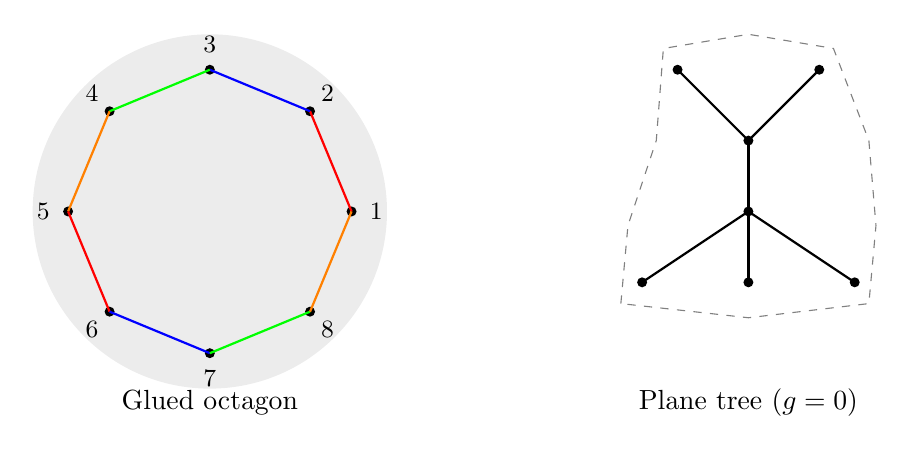
\begin{tikzpicture}[scale=0.9]

% ------------------------------------------------------------------
%  Left panel – Regular octagon whose edges are pair‑wise identified
% ------------------------------------------------------------------
\begin{scope}[xshift=-3.8cm]

  % Interior "surface" just for visual hint
  \fill[gray!15] (0,0) circle (2.5cm);

  % Vertices of the octagon
  \foreach \ang/\idx in {0/1,45/2,90/3,135/4,180/5,225/6,270/7,315/8}{
      \coordinate (v\idx) at (\ang:2cm);
      \fill (v\idx) circle (2pt);
      \node[font=\small] at (\ang:2.35cm) {\idx};
  }

  % Coloured, oriented edges (matching colours = glued pair)
  \foreach \a/\b/\clr in {1/2/red,2/3/blue,3/4/green,4/5/orange,
                          5/6/red,6/7/blue,7/8/green,8/1/orange}{
      \draw[thick,\clr] (v\a) -- (v\b);
  }

  % Sub‑caption
  \node at (0,-2.7) {Glued octagon};

\end{scope}

% ----------------------------------------------
%  Right panel – A representative plane tree
% ----------------------------------------------
\begin{scope}[xshift=3.8cm]

  % Edges of the tree
  \draw[thick] (0,0) -- (0,1);
  \draw[thick] (0,1) -- (-1,2);
  \draw[thick] (0,1) -- (1,2);
  \draw[thick] (0,0) -- (-1.5,-1);
  \draw[thick] (0,0) -- (0,-1);
  \draw[thick] (0,0) -- (1.5,-1);

  % Vertices
  \foreach \p in {(0,0),(0,1),(-1,2),(1,2),(-1.5,-1),(0,-1),(1.5,-1)}{
      \fill \p circle (2pt);
  }

  % Dashed outline of the single face
  \draw[gray,dashed]
        (-1.8,-1.3) -- (-1.7,-0.2) -- (-1.3,1) -- (-1.2,2.3) --
        (0,2.5) -- (1.2,2.3) -- (1.7,1) -- (1.8,-0.2) -- (1.7,-1.3) --
        (0,-1.5) -- cycle;

  % Sub‑caption
  \node at (0,-2.7) {Plane tree ($g=0$)};

\end{scope}
\end{tikzpicture}

\caption{A polygon whose edges are pairwise identified (indicated by matching colours) to form a one–face ribbon graph.  For genus~$0$ the result is a plane tree; for higher genus the same edge–pairing introduces handles on the underlying surface.}
\end{figure}

\subsection*{Haar Measure on $U(N)$ and Weingarten's Formula}

To make the above ideas precise, we need to compute integrals over the \textbf{Haar measure} on the unitary group $U(N)$. Recall:

\begin{definition}[Haar measure]
The \emph{Haar measure} $dU$ on $U(N)$ is the unique probability measure that is left- and right-invariant under the unitary group. In practice, sampling $U$ from Haar measure means $U$ is a ``random unitary matrix'' uniformly distributed with respect to the group's symmetries. Integration with respect to $dU$ corresponds to averaging over a Haar-random unitary matrix.
\end{definition}

We are interested in integrals of the form $\int_{U(N)} U_{i_1 j_1}U_{i_2 j_2}\cdots U_{i_m j_m} \,\overline{U_{k_1 l_1}U_{k_2 l_2}\cdots U_{k_m l_m}}\,dU$, which are expectations of products of matrix entries of $U$ and their complex conjugates. A fundamental result known as the \textbf{Weingarten formula} gives a complete answer in terms of the symmetric group $S_m$. It expresses the integral as a sum over all pairings of the $m$ ``$U$'' factors with the $m$ ``$\bar U$'' factors.

\begin{theorem}[Weingarten formula]
For any $m\ge 1$, and any indices $i_r,j_r,k_r,l_r$ ($1\le r \le m$), we have
\begin{equation}\label{eq:Weingarten}
\int_{U(N)} \prod_{r=1}^m U_{i_r j_r}\,\overline{U_{k_r l_r}}\;dU \;=\; \sum_{\sigma,\tau \in S_m} \;\prod_{r=1}^m \delta_{\,i_r,\,k_{\sigma(r)}}\,\delta_{\,j_r,\,l_{\tau(r)}}\;\;Wg_N(\sigma^{-1}\tau)\,,
\end{equation}
where $Wg_N(\pi)$ is the \emph{Weingarten function} on $S_m$, which depends only on the permutation $\pi=\sigma^{-1}\tau$ and $N$. In particular, $Wg_N(\pi)$ is the reciprocal of the dimension of the invariant subspace associated to $\pi$; it behaves like $O(N^{-m-|\pi|})$ for large $N$, with $|\pi|$ the number of disjoint cycles in $\pi$.
\end{theorem}

The formula \eqref{eq:Weingarten} may look complicated, but it simply encodes the fact that to get a nonzero integral, the indices $i_r$ must match up with the indices $k_s$ in some pairing (given by a permutation $\sigma$), and similarly $j_r$ must match $l_t$ according to some permutation $\tau$. Each such identification of indices contributes a delta Kronecker $\delta_{i_r,k_{s}}$. The weight $Wg_N(\sigma^{-1}\tau)$ can be thought of as a \emph{characteristic} of how the pairings $\sigma$ and $\tau$ interact. The Weingarten function is known explicitly in terms of representation theory of $S_m$ (through characters or Schur polynomials), but we will not need its precise form beyond small cases.

\begin{remark}
For $m=1$, there is only one permutation in $S_1$, and we obtain the basic orthonormality relation
\[ \int_{U(N)} U_{ij}\,\overline{U_{kl}}\;dU \;=\; \frac{1}{N}\,\delta_{i,k}\,\delta_{j,l}\,. \]
This reflects the fact that the rows (or columns) of a Haar unitary form an orthonormal basis in $\mathbb{C}^N$. For $m=2$, the sum in \eqref{eq:Weingarten} runs over the two permutations in $S_2$: the identity $e$ and the transposition $(1\,2)$. In this case one finds
\[ \int_{U(N)} U_{i_1 j_1} U_{i_2 j_2}\,\overline{U_{k_1 l_1} U_{k_2 l_2}}\;dU \;=\; \delta_{i_1,k_1}\delta_{i_2,k_2}\delta_{j_1,l_1}\delta_{j_2,l_2}\;-\;\frac{1}{N^2-1}\,\delta_{i_1,k_2}\delta_{i_2,k_1}\delta_{j_1,l_2}\delta_{j_2,l_1}\,. \]
Here the first term corresponds to $\sigma=\tau=e$ (pairing each $U$ with the corresponding $\bar U$), and the second term corresponds to $\sigma=(1\,2), \tau=e$ (pairing $U_{i_1 j_1}$ with $\bar U_{k_2 l_2}$ and $U_{i_2 j_2}$ with $\bar U_{k_1 l_1}$). The coefficient $-1/(N^2-1)$ is the Weingarten function value $Wg_N((1\,2))$ for the transposition in $S_2$. We see the $1/N^2$ suppression of the ``crossing'' term, which will be crucial for genus expansions.
\end{remark}

The takeaway is that \textbf{integrals over Haar-random unitaries reduce to sums over permutations (pairings)}. Diagrammatically, one can represent each $U_{i_r j_r}$ as a directed edge carrying an index $i_r$ at one end and $j_r$ at the other; similarly $\overline{U_{k_s l_s}}$ is an oppositely directed edge with $k_s$ and $l_s$ at its ends. The delta functions $\delta_{i_r,k_{\sigma(r)}}$ in \eqref{eq:Weingarten} mean that we identify the end of $U_{i_r j_r}$ with the end of $\overline{U_{k_s l_s}}$ having the same index. Thus each term in the sum over $\sigma,\tau$ describes a way to \textbf{glue $m$ ``prongs'' to $m$ ``sockets''}, producing a closed pairing of $m$ $U$-edges with $m$ $\bar U$-edges. These pairings are in bijection with \textbf{ribbon graph structures}. Indeed, when we contract matching indices, the $U$ edges and $\bar U$ edges join up to form cycles; because $U$ indices $i_r$ are identified with $k_{\sigma(r)}$ and $U$ indices $j_r$ with $l_{\tau(r)}$, the result is a permutation pairing that can be visualized on a surface. The power of the Weingarten formula is that it counts all such pairings with the correct weight. In the next section, we apply this formula to the specific case of interest: the \textbf{unitary matrix integral that counts one-face maps}.

\subsection*{Harer–Zagier Formula for One-Face Maps}

We now focus on a particular observable that generates one-face maps: the product of a trace and its conjugate. Consider
\[ X_n \;:=\; \operatorname{Tr}(U^n)\,\overline{\operatorname{Tr}(U^n)} \;=\; \operatorname{Tr}(U^n)\,\operatorname{Tr}((U^*)^n)\,. \]
Expanding this out in indices:
\[ \operatorname{Tr}(U^n) = \sum_{a_1,\dots,a_n=1}^N U_{a_1 a_2} U_{a_2 a_3}\cdots U_{a_n a_1}, \]
\[ \operatorname{Tr}((U^*)^n) = \sum_{b_1,\dots,b_n=1}^N \overline{U_{b_1 b_2} U_{b_2 b_3}\cdots U_{b_n b_1}} = \sum_{b_1,\dots,b_n} \overline{U_{b_1 b_2}}\,\overline{U_{b_2 b_3}}\cdots \overline{U_{b_n b_1}}. \]
Thus $X_n = \sum_{a_\bullet,b_\bullet} U_{a_1 a_2}\cdots U_{a_n a_1}\,\overline{U_{b_1 b_2}\cdots U_{b_n b_1}}$. This is precisely of the form covered by the Weingarten formula \eqref{eq:Weingarten}, with $m=n$ and the $U$ indices $(i_1,\dots,i_n)$ identified as $(a_1,a_2,\dots,a_n)$ and $(j_1,\dots,j_n)=(a_2,a_3,\dots,a_1)$, and similarly $(k_1,\dots,k_n)=(b_1,b_2,\dots,b_n)$ and $(l_1,\dots,l_n)=(b_2,b_3,\dots,b_1)$. The delta constraints in \eqref{eq:Weingarten} enforce that after integration, $a_\bullet$ and $b_\bullet$ indices must match in a way that corresponds to a permutation pairing of the $n$-gon formed by the $U$ factors with the $n$-gon formed by the $\bar U$ factors. In other words, each term in $\mathbb{E}[X_n] = \int X_n\,dU$ can be visualized as gluing the edges of a $2n$-gon (with $n$ oriented edges from the $U^n$ trace and $n$ from the $(U^*)^n$ trace) according to some identification pattern. The result of a given gluing is a connected ribbon graph with one face (since the $2n$-gon's boundary becomes a single closed curve once all pairs of edges are glued). See the figure below for an illustration.

By this reasoning, we expect
\[ \mathbb{E}_{U(N)}[\,X_n\,] \;=\; \sum_{\text{pairings }P \text{ of }2n\text{-gon}} N^{-\alpha(P)}, \]
where each pairing $P$ produces a one-face map of some genus $g$, and contributes a factor $N^{-2g}$ (up to an overall power of $N$) from the Weingarten weights. In fact, one can show that
\[ \mathbb{E}[X_n] = \sum_{g=0}^{\lfloor n/2\rfloor} \epsilon_g(n)\; N^{\,1-2g}. \]
The power of $N$ reflects the fact that each handle (genus increment) in the surface comes with a factor $1/N^2$. The leading power of $N$ is $N^1$ for $g=0$ (planar case), then $N^{-1}$ for $g=1$, etc. The $N^1$ rather than $N^0$ for planar is because we are counting \emph{one-face} maps which have $F=1$; more precisely, $\mathbb{E}[X_n] = N\,\epsilon_0(n) + N^{-1}\epsilon_1(n) + \cdots + N^{1-2\lfloor n/2\rfloor}\,\epsilon_{\lfloor n/2\rfloor}(n)$. One can divide by $N$ if desired to get a symmetric $N^{ -2g}$ expansion. In any case, the coefficients $\epsilon_g(n)$ are exactly the numbers of one-face maps we want to determine.

Harer and Zagier in 1986 derived a beautiful closed-form description of these coefficients. To state their formula, it is convenient to introduce the double factorial notation $(2n-1)!! = 1\cdot 3 \cdot 5 \cdots (2n-1)$ (the number of ways to pair up $2n$ objects). They proved:

\begin{theorem}[Harer–Zagier formula]\label{thm:HZ}
The numbers $\epsilon_g(n)$ of genus-$g$ one-face maps with $n$ edges satisfy the generating function identity
\begin{equation}\label{eq:HZgen}
1 \;+\; 2\sum_{n\ge 1}\sum_{g\ge 0} \epsilon_g(n)\,\frac{x^{\,n+1}}{(2n-1)!!}\,y^{\,n+1-2g} \;=\; \Big( \frac{1 + x}{\,1 - x\,}\Big)^{\,y}\,,
\end{equation}
as an equality of formal power series in $x$ and $y$. Equivalently, for each fixed $n\ge 1$, $\epsilon_g(n)$ is zero for $g > \lfloor n/2\rfloor$ and one has the explicit formula (obtained by expanding the right-hand side of \eqref{eq:HZgen}):
\[ \epsilon_g(n) \;=\; (2n-1)!! \sum_{j=0}^{n+1-2g} (-1)^j \binom{n+1-2g}{j}\binom{n+1+j}{\,j\,}\,. \]
\end{theorem}

While the form of \eqref{eq:HZgen} may appear daunting, it encodes a great deal of structure. Let's unpack it step by step:

- First, setting $y=1$ in \eqref{eq:HZgen} (which sums over all genera) gives
\[ 1 + 2\sum_{n\ge 1} \frac{(2n-1)!!}{(2n-1)!!} x^{\,n+1} = \frac{1+x}{1-x}\,. \]
This reduces to the trivial identity $1 + 2\sum_{n\ge 1} x^{n+1} = \frac{1+x}{1-x}$, since $(2n-1)!!/(2n-1)!!=1$. More interestingly, the coefficient extraction here confirms that
\[ \sum_{g\ge 0} \epsilon_g(n) = (2n-1)!!, \]
i.e. the total number of one-face maps with $n$ edges (summing over all possible genera) is $(2n-1)!!$. This matches our intuition that any pairing of the $2n$ sides of a $2n$-gon yields some surface. For small $n$, $(2n-1)!!$ grows quickly: for $n=1,2,3,4,\dots$ we have $1, 3, 15, 105, \dots$.

- Next, the exponent $y$ on the right side of \eqref{eq:HZgen} allows one to isolate the contributions of a given genus. Expanding $(\frac{1+x}{1-x})^y$ formally in $y$ yields the binomial coefficients in the explicit formula above. In particular, one can extract a \textbf{recurrence relation} from \eqref{eq:HZgen} by comparing coefficients of $y^{\,n+1-2g}x^{\,n+1}$ on both sides. Doing so yields a \emph{three-term recurrence} for $\epsilon_g(n)$ (in $n$) relating $\epsilon_g(n)$, $\epsilon_g(n-1)$, and $\epsilon_{g-1}(n-1)$. We omit the algebraic details here (they were part of Harer–Zagier's original derivation), but we will \emph{derive} this recurrence combinatorially in the next section.

- Finally, setting $y= n+1-2g$ (formally) in \eqref{eq:HZgen} one can solve for $\epsilon_g(n)$ directly. The given explicit sum is one convenient form of the answer. While the summation formula may not look obviously positive, it indeed evaluates to a nonnegative integer for all valid $n,g$. These numbers start as follows: for $n=1$, $\epsilon_0(1)=1$ (a single edge on a sphere, which is a loop, counted as a plane tree with one edge) and $\epsilon_g(1)=0$ for $g\ge 1$. For $n=2$, $\epsilon_0(2)=2$, $\epsilon_1(2)=1$ (as $1+2=3=(2\cdot2-1)!!$), and higher $g$ zero. For $n=3$, $\epsilon_0(3)=5$, $\epsilon_1(3)=10$ (since $5+10=15=(5)!!$), $\epsilon_2(3)=0$. For $n=4$, one finds $\epsilon_0(4)=14$, $\epsilon_1(4)=56$, $\epsilon_2(4)=35$ (indeed $14+56+35=105=(7)!!$), and so on. The planar numbers $\epsilon_0(n)$ are well-known Catalan numbers, and the higher-genus ones can be identified with other combinatorial sequences.

\begin{remark}
In the planar case $g=0$, the Harer–Zagier formula reduces to $\epsilon_0(n) = \frac{1}{n+1}\binom{2n}{n}$. This is the $n$th \textbf{Catalan number}. Planar one-face maps are in bijection with plane trees (think of the unique face as the outside region of a tree drawn on the sphere), and indeed the number of (rooted) plane trees with $n$ edges is the Catalan number $C_n$. For example, $\epsilon_0(2)=2$ corresponds to the two distinct plane trees with 2 edges. The fact that $\epsilon_0(n)$ is Catalan while $\sum_g \epsilon_g(n)=(2n-1)!!$ (which is much larger for $n>2$) reflects that most pairings of $2n$ edges produce surfaces of higher genus (many ``crossings''), whereas only a subset of ``non-crossing'' pairings produce a planar embedding. The numbers for $g>0$ do not have such a simple closed form name, but they grow rapidly with $n$ and $g$.
\end{remark}

Thus, $\mathbb{E}[\operatorname{Tr}(U^n)\overline{\operatorname{Tr}(U^n)}]$ is completely determined: it equals the polynomial in $N$ given by $\sum_{g=0}^{\lfloor n/2\rfloor}\epsilon_g(n) N^{\,1-2g}$. The leading term (as $N\to\infty$) is $\epsilon_0(n)N$, and the subleading corrections at order $N^{-1}, N^{-3},\dots$ carry the higher-genus information.

\subsection*{Genus Expansions and the $1/N$ Topological Expansion}

One of the most important insights from random matrix theory is that integrals like the above admit a \textbf{genus expansion} for large matrix size $N$. In our case, the Harer–Zagier formula explicitly gives such an expansion:
\[ \mathbb{E}_{U(N)}[X_n] \;=\; \epsilon_0(n)\,N \;+\; \epsilon_1(n)\,\frac{1}{N} \;+\; \epsilon_2(n)\,\frac{1}{N^3} \;+\; \cdots, \]
with only powers $N^{1-2g}$ appearing. This is a special case of a general phenomenon. For many random matrix ensembles, the expectation of a normalized trace (or product of traces) can be expanded in a power series in $1/N^2$, where the coefficient of $1/N^{2g}$ is enumerating graphs of genus $g$. This is often called the \textbf{$1/N$ expansion} or \textbf{'t Hooft expansion}.

In the present context, if we define $W_n(N) := \frac{1}{N}\mathbb{E}[\operatorname{Tr}(U^n)\overline{\operatorname{Tr}(U^n)}]$, then $W_n(N) = \epsilon_0(n) + \epsilon_1(n)N^{-2} + \epsilon_2(n)N^{-4} + \cdots$. In the limit $N\to\infty$, $W_n(N)$ approaches $\epsilon_0(n)$, recovering the fact that planar diagrams dominate at large $N$. The corrections of order $1/N^2$ correspond to adding handles to the surface, which are suppressed for large but finite $N$.

This topological $1/N^2$ expansion was first exploited by 't Hooft in the context of gauge theory (1974) and was later widely used in matrix models for gravity. In our case, we see it explicitly in the formula for $\mathbb{E}[X_n]$. Each power of $1/N^2$ is tied to the Euler characteristic of the ribbon graph (since for a one-face map, $\chi = 2-2g$, and the contribution goes like $N^{\chi} = N^{2-2g}$ up to the $N^1$ normalization needed for one face). If we had a random matrix integral generating maps with $F$ faces, the leading power would be $N^F$ and the expansion would involve $N^{2-2g - F}$.

In summary, \textbf{large-$N$ matrix integrals enumerate surfaces by genus}. The Harer–Zagier result is a concrete instance of this: it tells us exactly how many genus-$g$ surfaces (with one boundary) contribute to the unitary integral. This linkage between algebraic integrals and topological counting is a cornerstone of \textbf{random matrix theory in mathematical physics}, providing a bridge between probability and topology.

\subsection*{Recursion via Chord Diagrams: Proof Outline of Harer–Zagier}

We now outline a combinatorial proof of Theorem \ref{thm:HZ} by interpreting one-face maps as chord diagrams and finding a recurrence. This approach was hinted at above in deriving the structure of the Weingarten expansion, but here we make it into a rigorous counting argument.

Represent a one-face map with $n$ edges by a $2n$-gon whose edges are labeled in pairs: each pair of identical labels indicates that those two edges are glued together in the map. Since the map has one face, the $2n$-gon's entire boundary is traversed once (before gluing). Another convenient representation is a \textbf{chord diagram}: place $2n$ points around a circle (these represent the midpoints of the $2n$ edges of the polygon), and connect each pair of identical labels by a chord inside the circle. Every way to connect $2n$ points in pairs by chords corresponds to a (not necessarily planar) one-face map. For example, for $n=3$ one such pairing might connect points $(1,4), (2,6), (3,5)$ (assuming points labeled $1$ through $6$ around the circle); this particular chord diagram has one crossing of chords (and corresponds to a genus $1$ map).

To derive a recurrence, \textbf{pick a distinguished edge} (or equivalently, point on the circle) and consider how its pairing looks. Without loss of generality, label one particular boundary edge as ``edge 1'' with endpoints (points) $A$ and $B$ on the circle. There are two cases for how edge 1 is glued (paired):

- \textbf{Case 1: Edge 1 is paired with an adjacent edge.} In the chord diagram, this means points $A$ and $B$ are next to each other around the circle and are directly connected by a chord. Gluing this pair of adjacent edges produces a ``handle-less'' identification: it does not introduce any crossing with other chords. Topologically, cutting edge 1 out of the map (removing that chord) leaves a one-face map with $n-1$ edges on the \emph{same genus} $g$. (In terms of the polygon, if two consecutive sides are glued, one can remove them and collapse the polygon, effectively reducing the problem to $2(n-1)$ sides without changing the genus.) There are $2n-1$ possible partner edges for edge 1 in total, but only \textbf{one} of them is the adjacent edge along the circle. Thus there is a unique pairing in this case (for each fixed edge 1): namely, $(A,B)$ itself.

- \textbf{Case 2: Edge 1 is paired with a non-adjacent edge.} That is, in the chord diagram the chord connecting $A$ to $B$ goes across the circle and \emph{crosses} some other chords. Equivalently, in the polygon picture, edge 1 is glued to some other edge that is not its immediate neighbor on the boundary. This operation \textbf{introduces a handle}: if the original map has genus $g$, then cutting along this chord will split the surface into two pieces, one of which is a one-face map of genus $g-1$ with fewer edges. In fact, removing a non-adjacent pair causes the genus to drop by 1 (because we essentially undo one handle). Combinatorially, suppose edge 1 (point $A$) is paired with another point $C$ that is not adjacent. This chord $(A,C)$ divides the $2n$ points on the circle into two arcs: one arc between $A$ and $C$ (moving clockwise, say) and the other between $C$ and $A$. These two arcs contain an even number of points in total (because excluding $A$ and $C$, there are $2n-2$ other points). The chords connecting the points on each arc among themselves form two smaller one-face maps, whose genera sum to $g-1$. But since our map is connected and has one face, one of those arcs must contain no other chord entirely inside it (all other chords must cross the chord $(A,C)$ to connect points from one arc to the
























\appendix
\setcounter{section}{14}

\section{Problems (due 2025-04-29)}





\bibliographystyle{alpha}
\bibliography{bib}


\medskip

\textsc{L. Petrov, University of Virginia, Department of Mathematics, 141 Cabell Drive, Kerchof Hall, P.O. Box 400137, Charlottesville, VA 22904, USA}

E-mail: \texttt{lenia.petrov@gmail.com}


\end{document}
